\chapter{Aufgabe 7}
\section{Aufgabe 7.1}
\paragraph{Aufgabenstellung}
Stellen Sie das Multimeter auf Widerstandsmessung ein und messen Sie den Widerstand des Steckbrettes indem Sie, wie in Abbildung 3 gezeigt, zwei Kabel in zwei verbundene Löcher stecken.

\begin{figure}
	\begin{minipage}[c]{0.48\linewidth}
		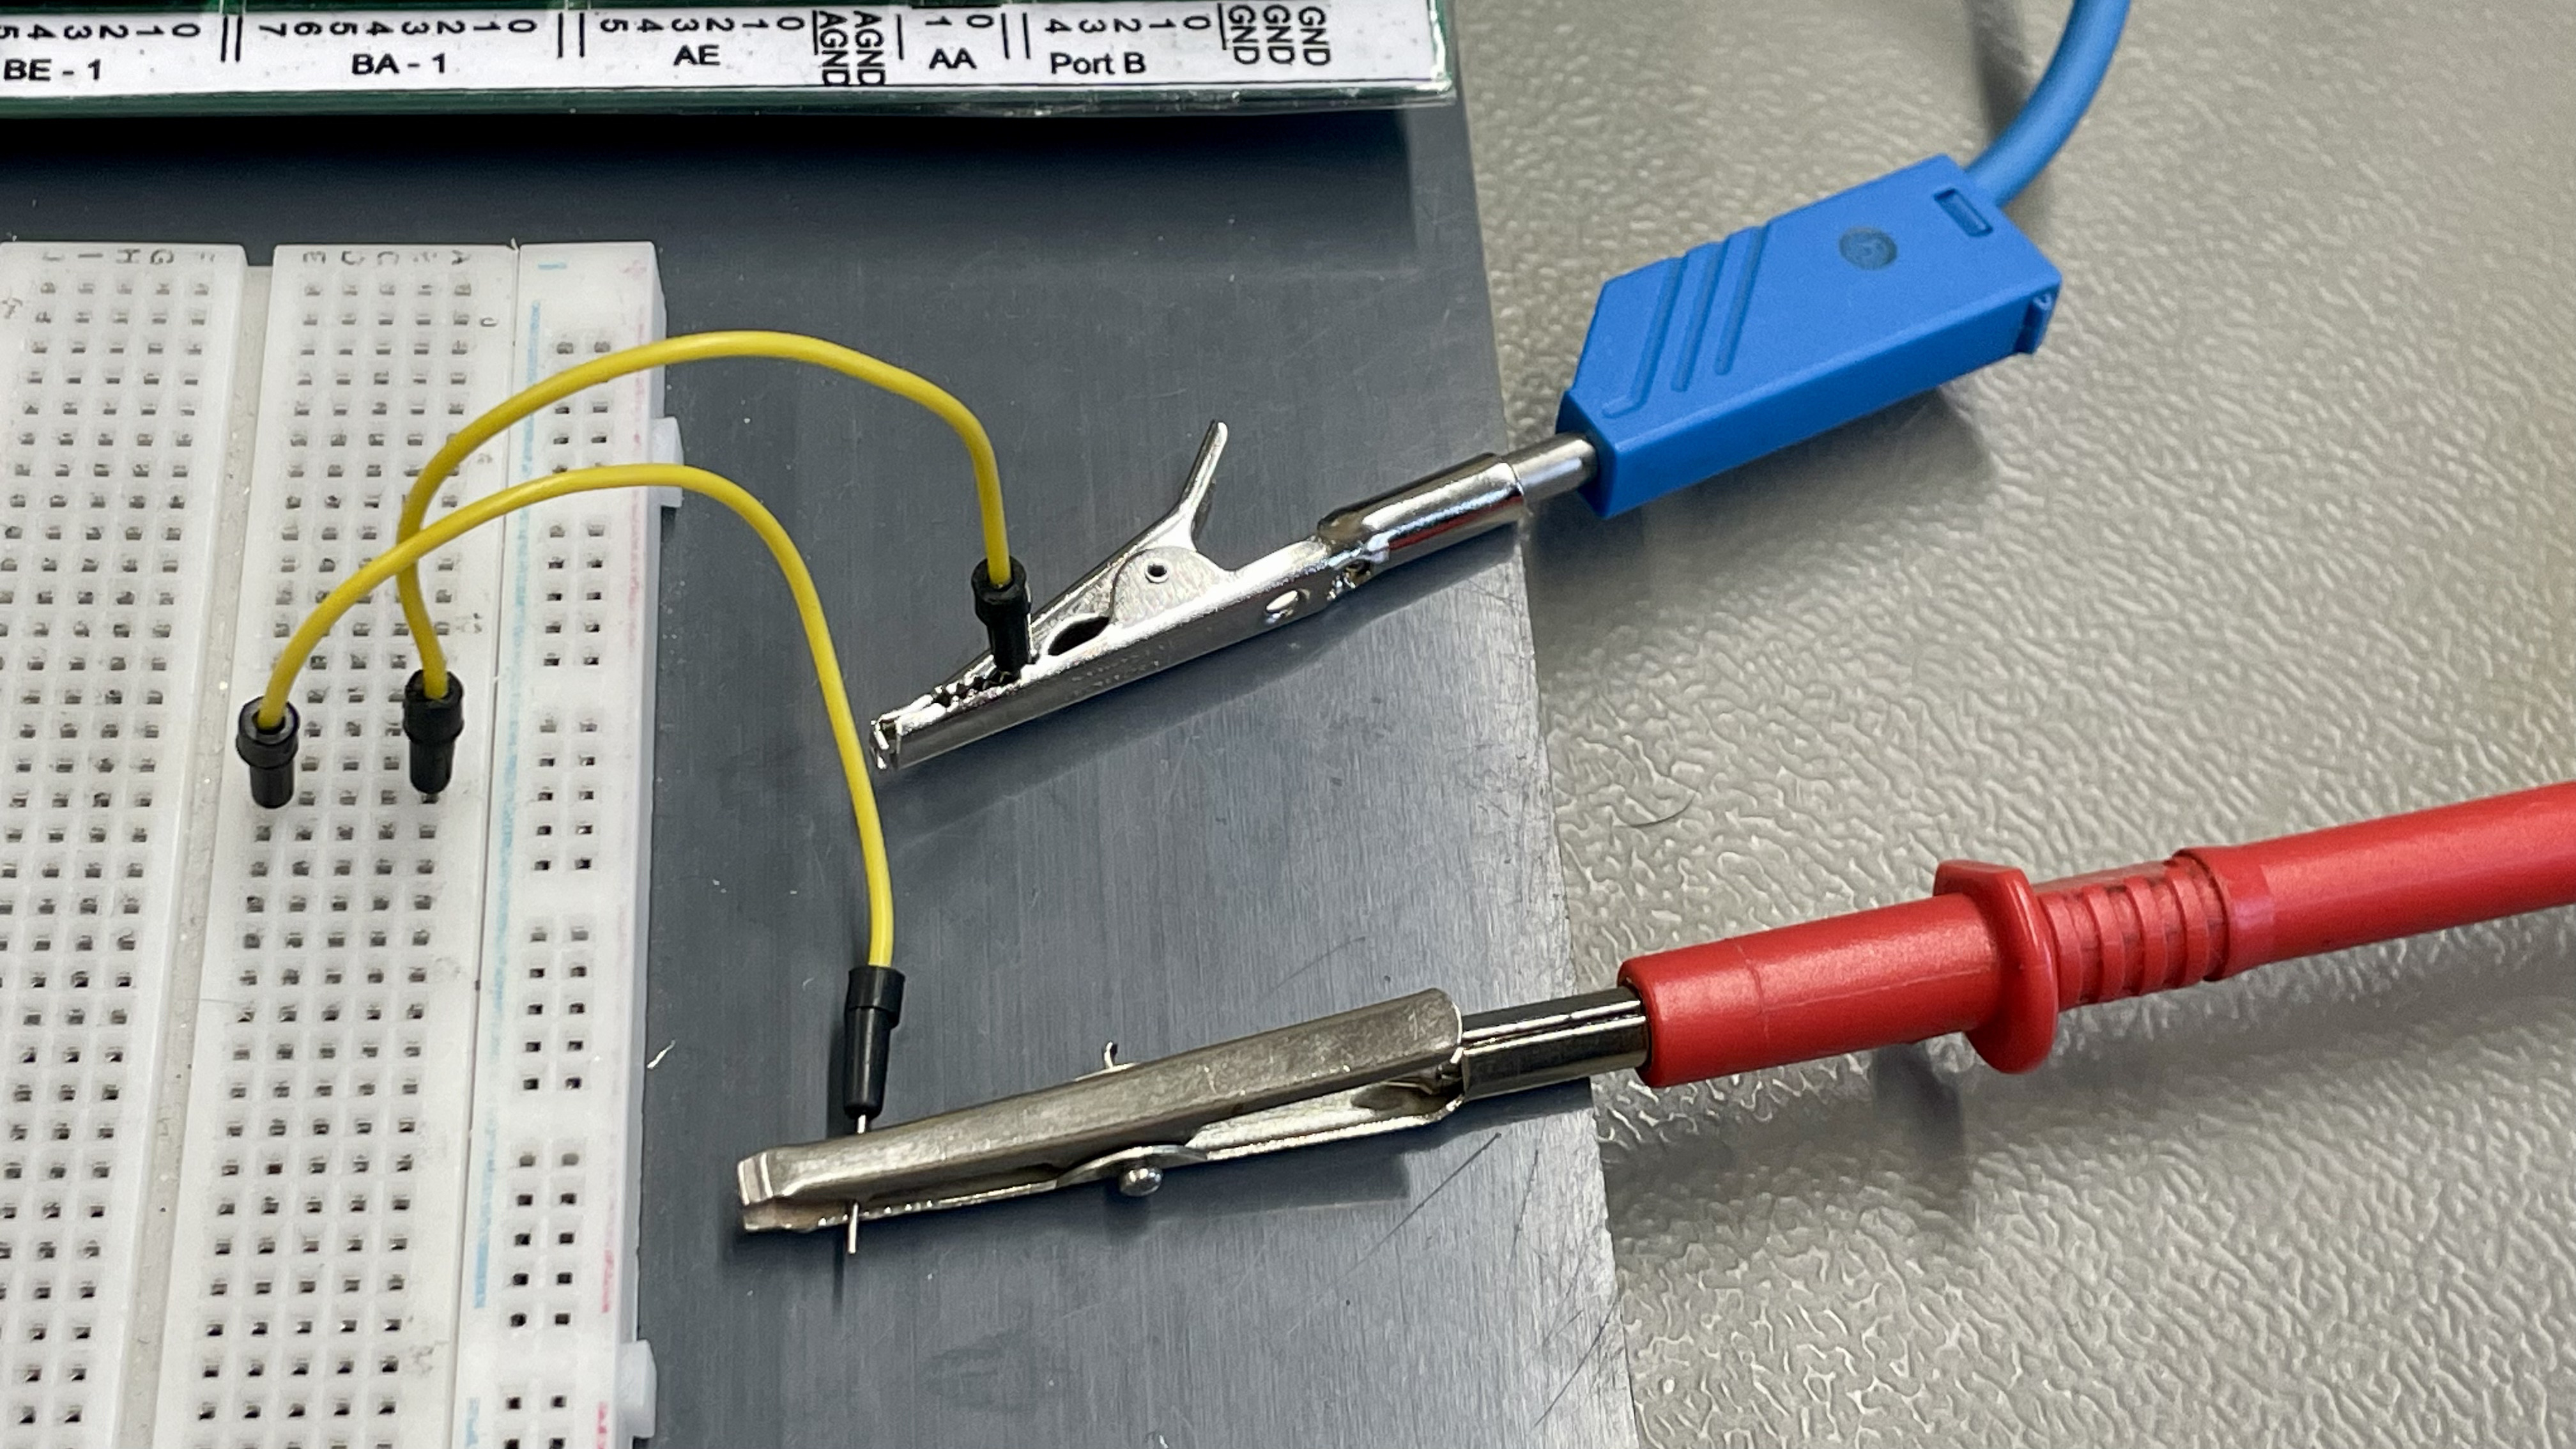
\includegraphics[width=\linewidth]{task7-1-0.jpg}
		\caption{Aufbau Widerstandsmessung}
		\label{task7-1-0}
	\end{minipage}
	\hfill
	\begin{minipage}[c]{0.485\linewidth}
		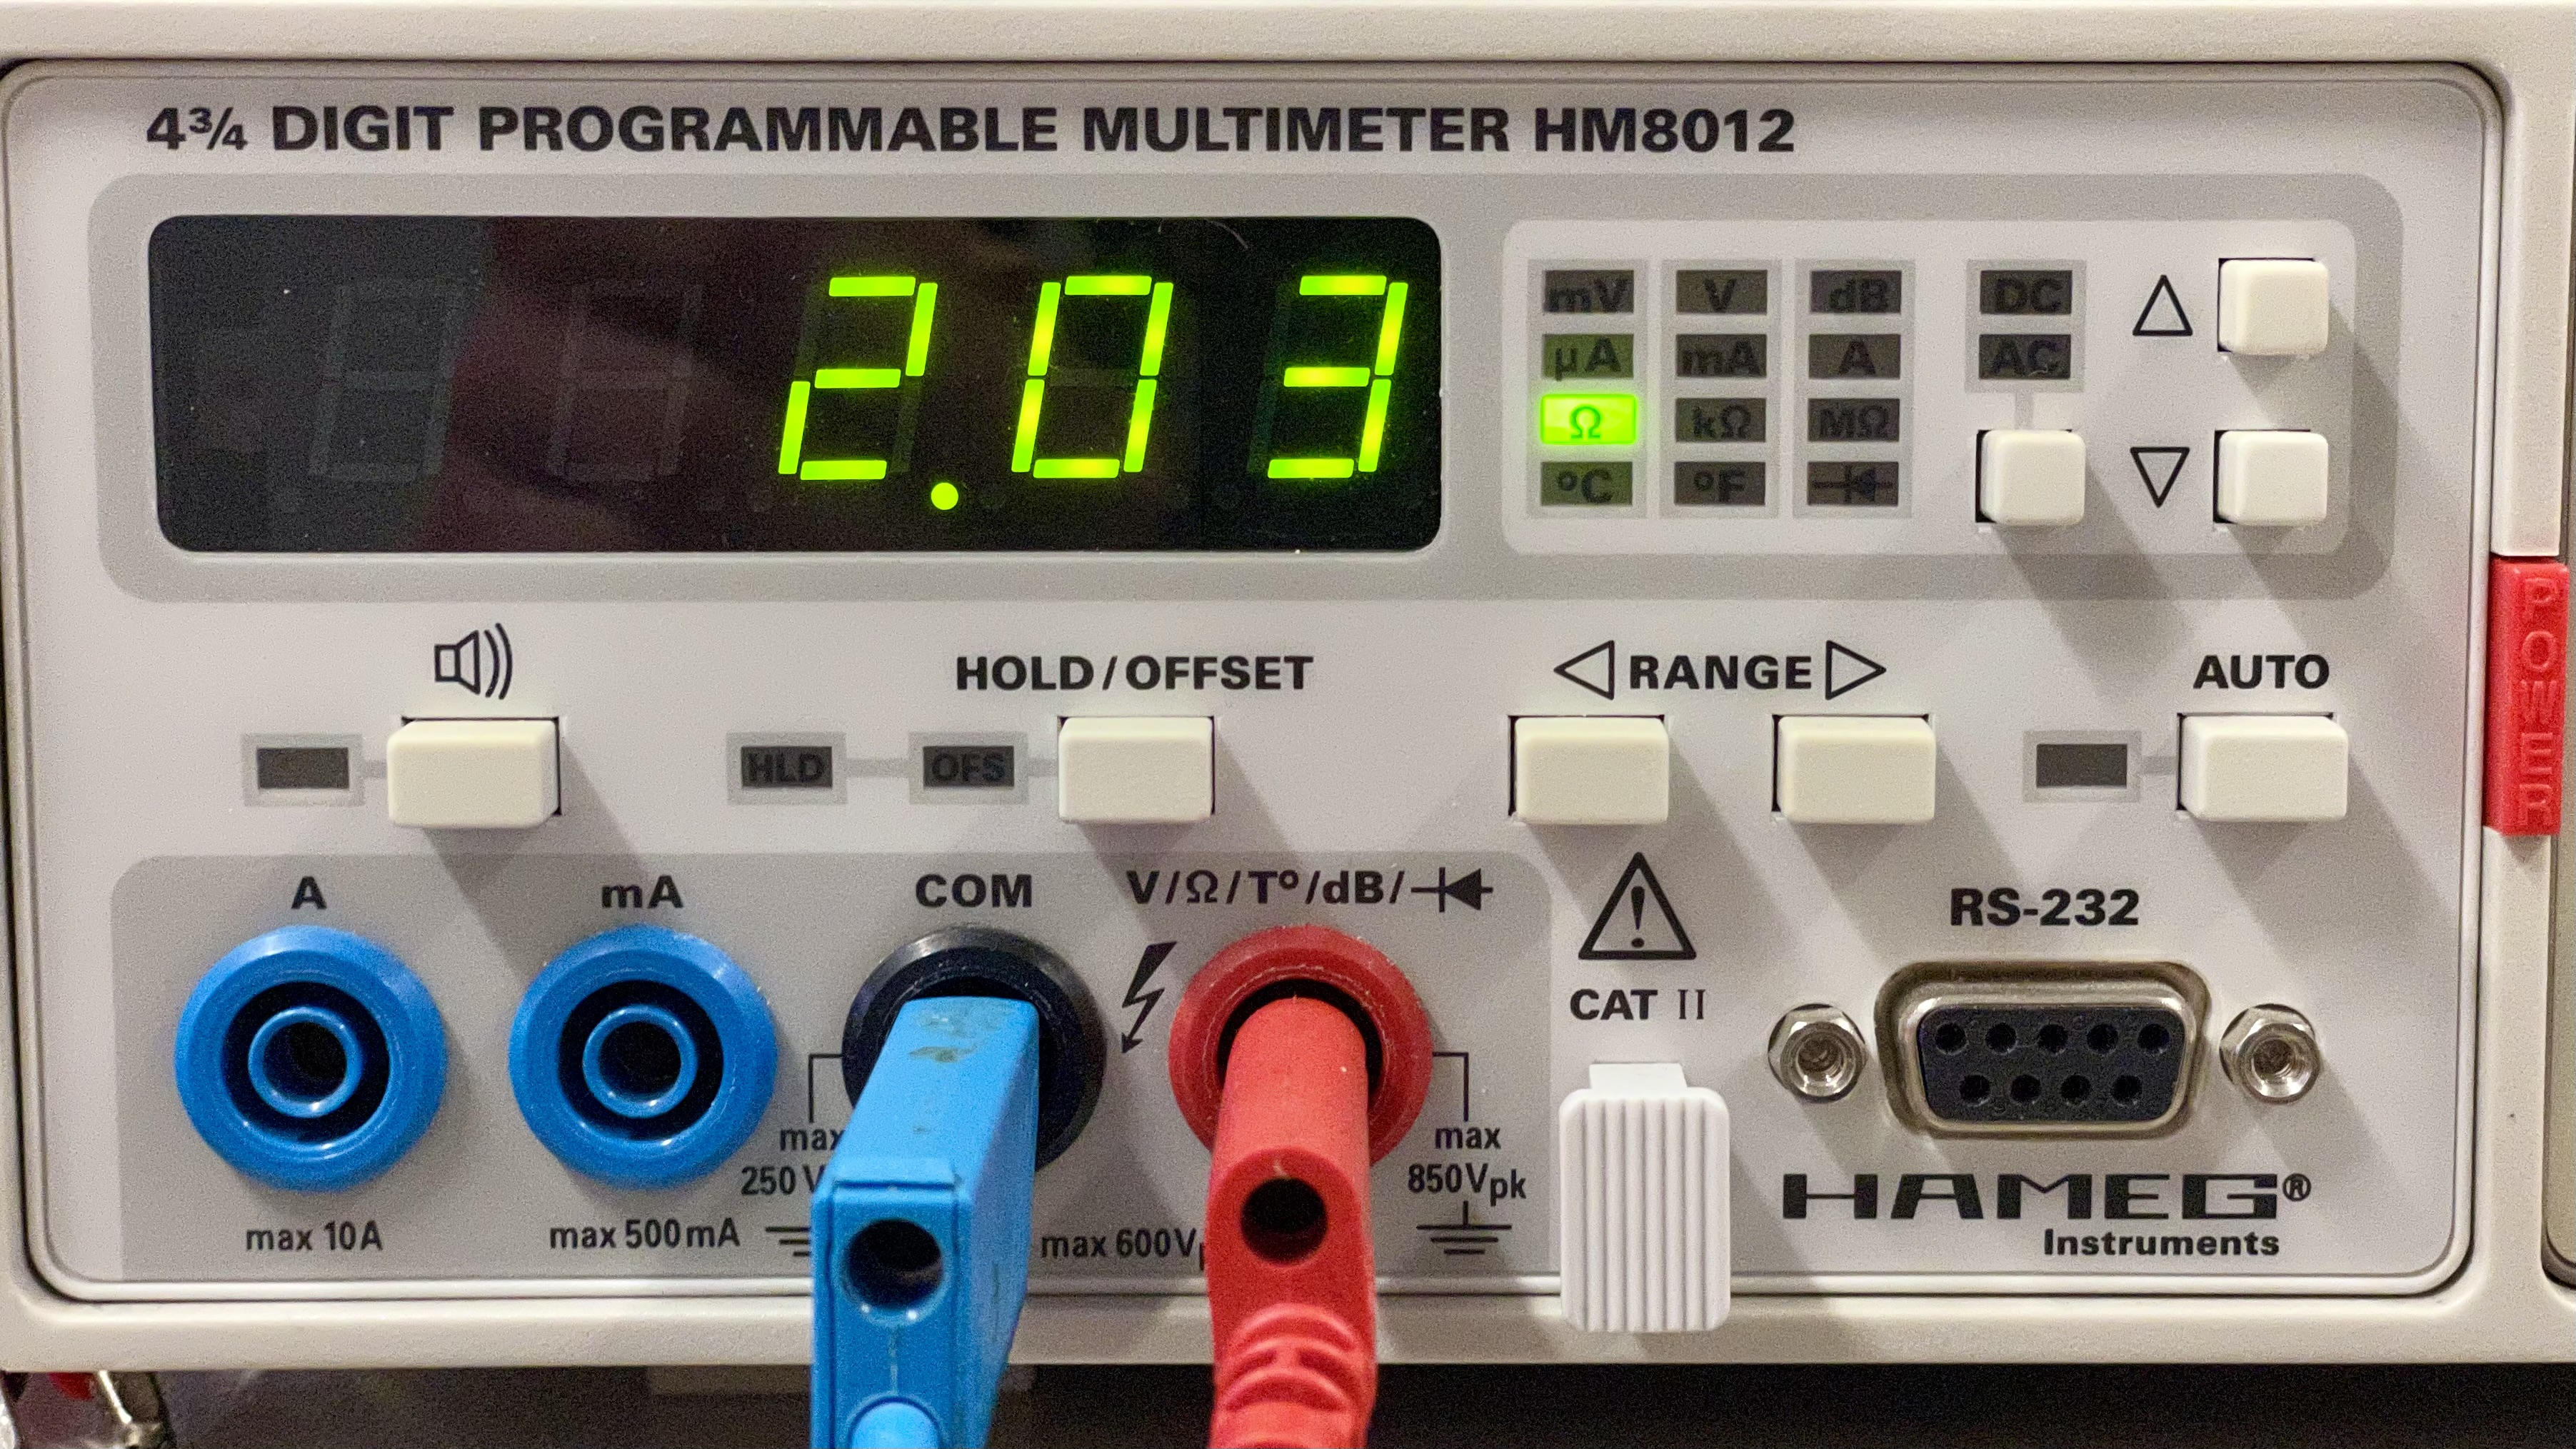
\includegraphics[width=\linewidth]{task7-1-1.jpg}
		\caption{Messung des Widerstands}
		\label{task7-1-1}
	\end{minipage}
	\label{task7-1}
\end{figure}

\paragraph{Durchführung}
Das Multimeter wird auf Widerstandsmessung eingestellt un an den entsprechenden Buchsen mit den Kabel zum Steckbrett verbunden. Auf dem Steckbrett führen die Kabel in die jeweils äußeren Steckplätze einer Kurzen leiste (Abbildung \vref{task7-1-0}). Das Multimeter zeigt \SI{2,03}{\ohm} an, wie in Abbildung \vref{task7-1-1} zu erkennen ist.

\paragraph{Schlussfolgerung}
Die Messung liefert ein plausibles Ergebnis.

\section{Aufgabe 7.2}
\paragraph{Aufgabenstellung}
Entscheiden Sie an welchen Stellen Sie in Schaltung Abb. 4 ein Voltmeter bzw. ein Amperemeter einsetzen. Messen Sie Strom und Spannung!

\paragraph{Vorüberlegung}
Stromstärke wird in Reihe geschaltet gemessen und Stromspannung parallel.

\paragraph{Durchführung}
Messpunkt 1 ist in Reihe geschaltet, daher wird hier die Stärke gemessen. Messpunkt 2 ist zu R1 und Messpunkt 3 zusätzlich noch zu R2 parallel geschaltet, daher wird hier die Spannung gemessen. Der Aufbau für alle drei Messpunkte kann Abbildung \vref{task7-2-1-aufbau} entnommen werden. Die Messwerte lauten \SI{44.97}{\milli\ampere} für Punkt 1, \SI{2,6}{\volt} für Punkt 2 und \SI{5,3}{\volt} für Punkt 3, wie Abbildung \vref{task7-2-1-messwerte} zeigt.

\begin{figure}
	\begin{minipage}[c]{0.32\linewidth}
		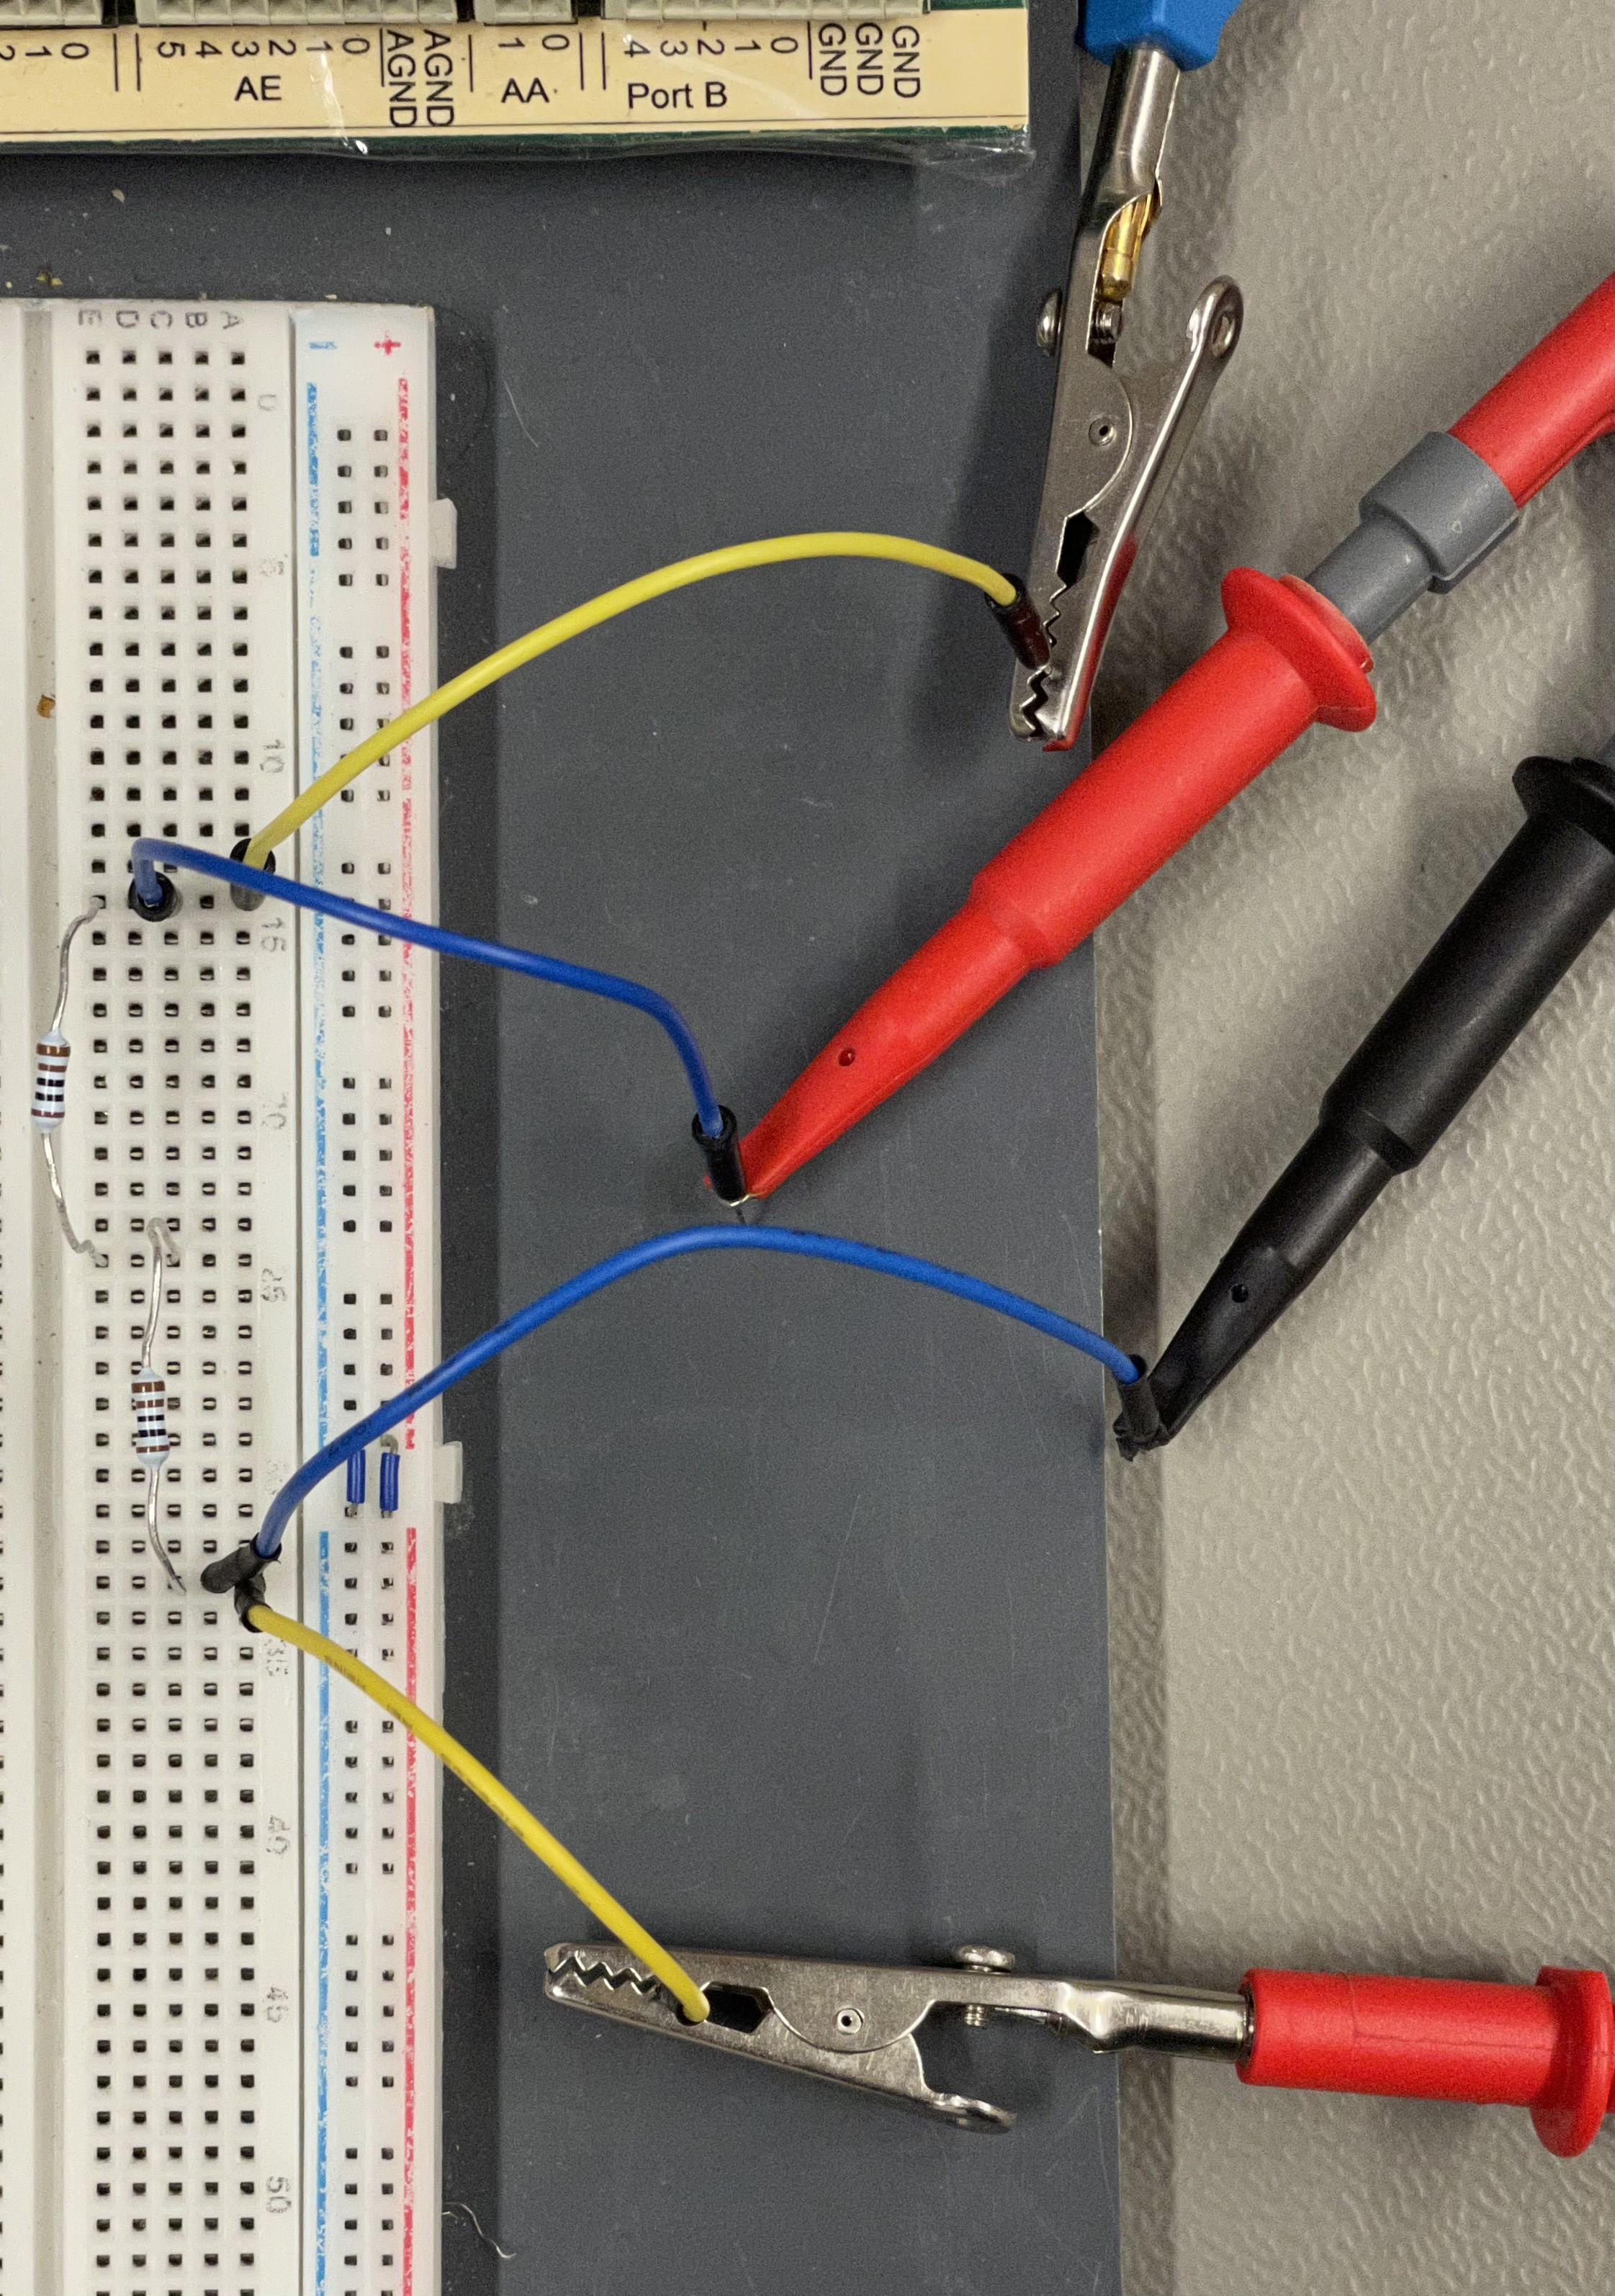
\includegraphics[width=\linewidth]{task7-2-1-0.JPG}
		\caption{Messpunkt 1}
		\label{task7-2-1-0}
	\end{minipage}
	\hfill
	\begin{minipage}[c]{0.32\linewidth}
		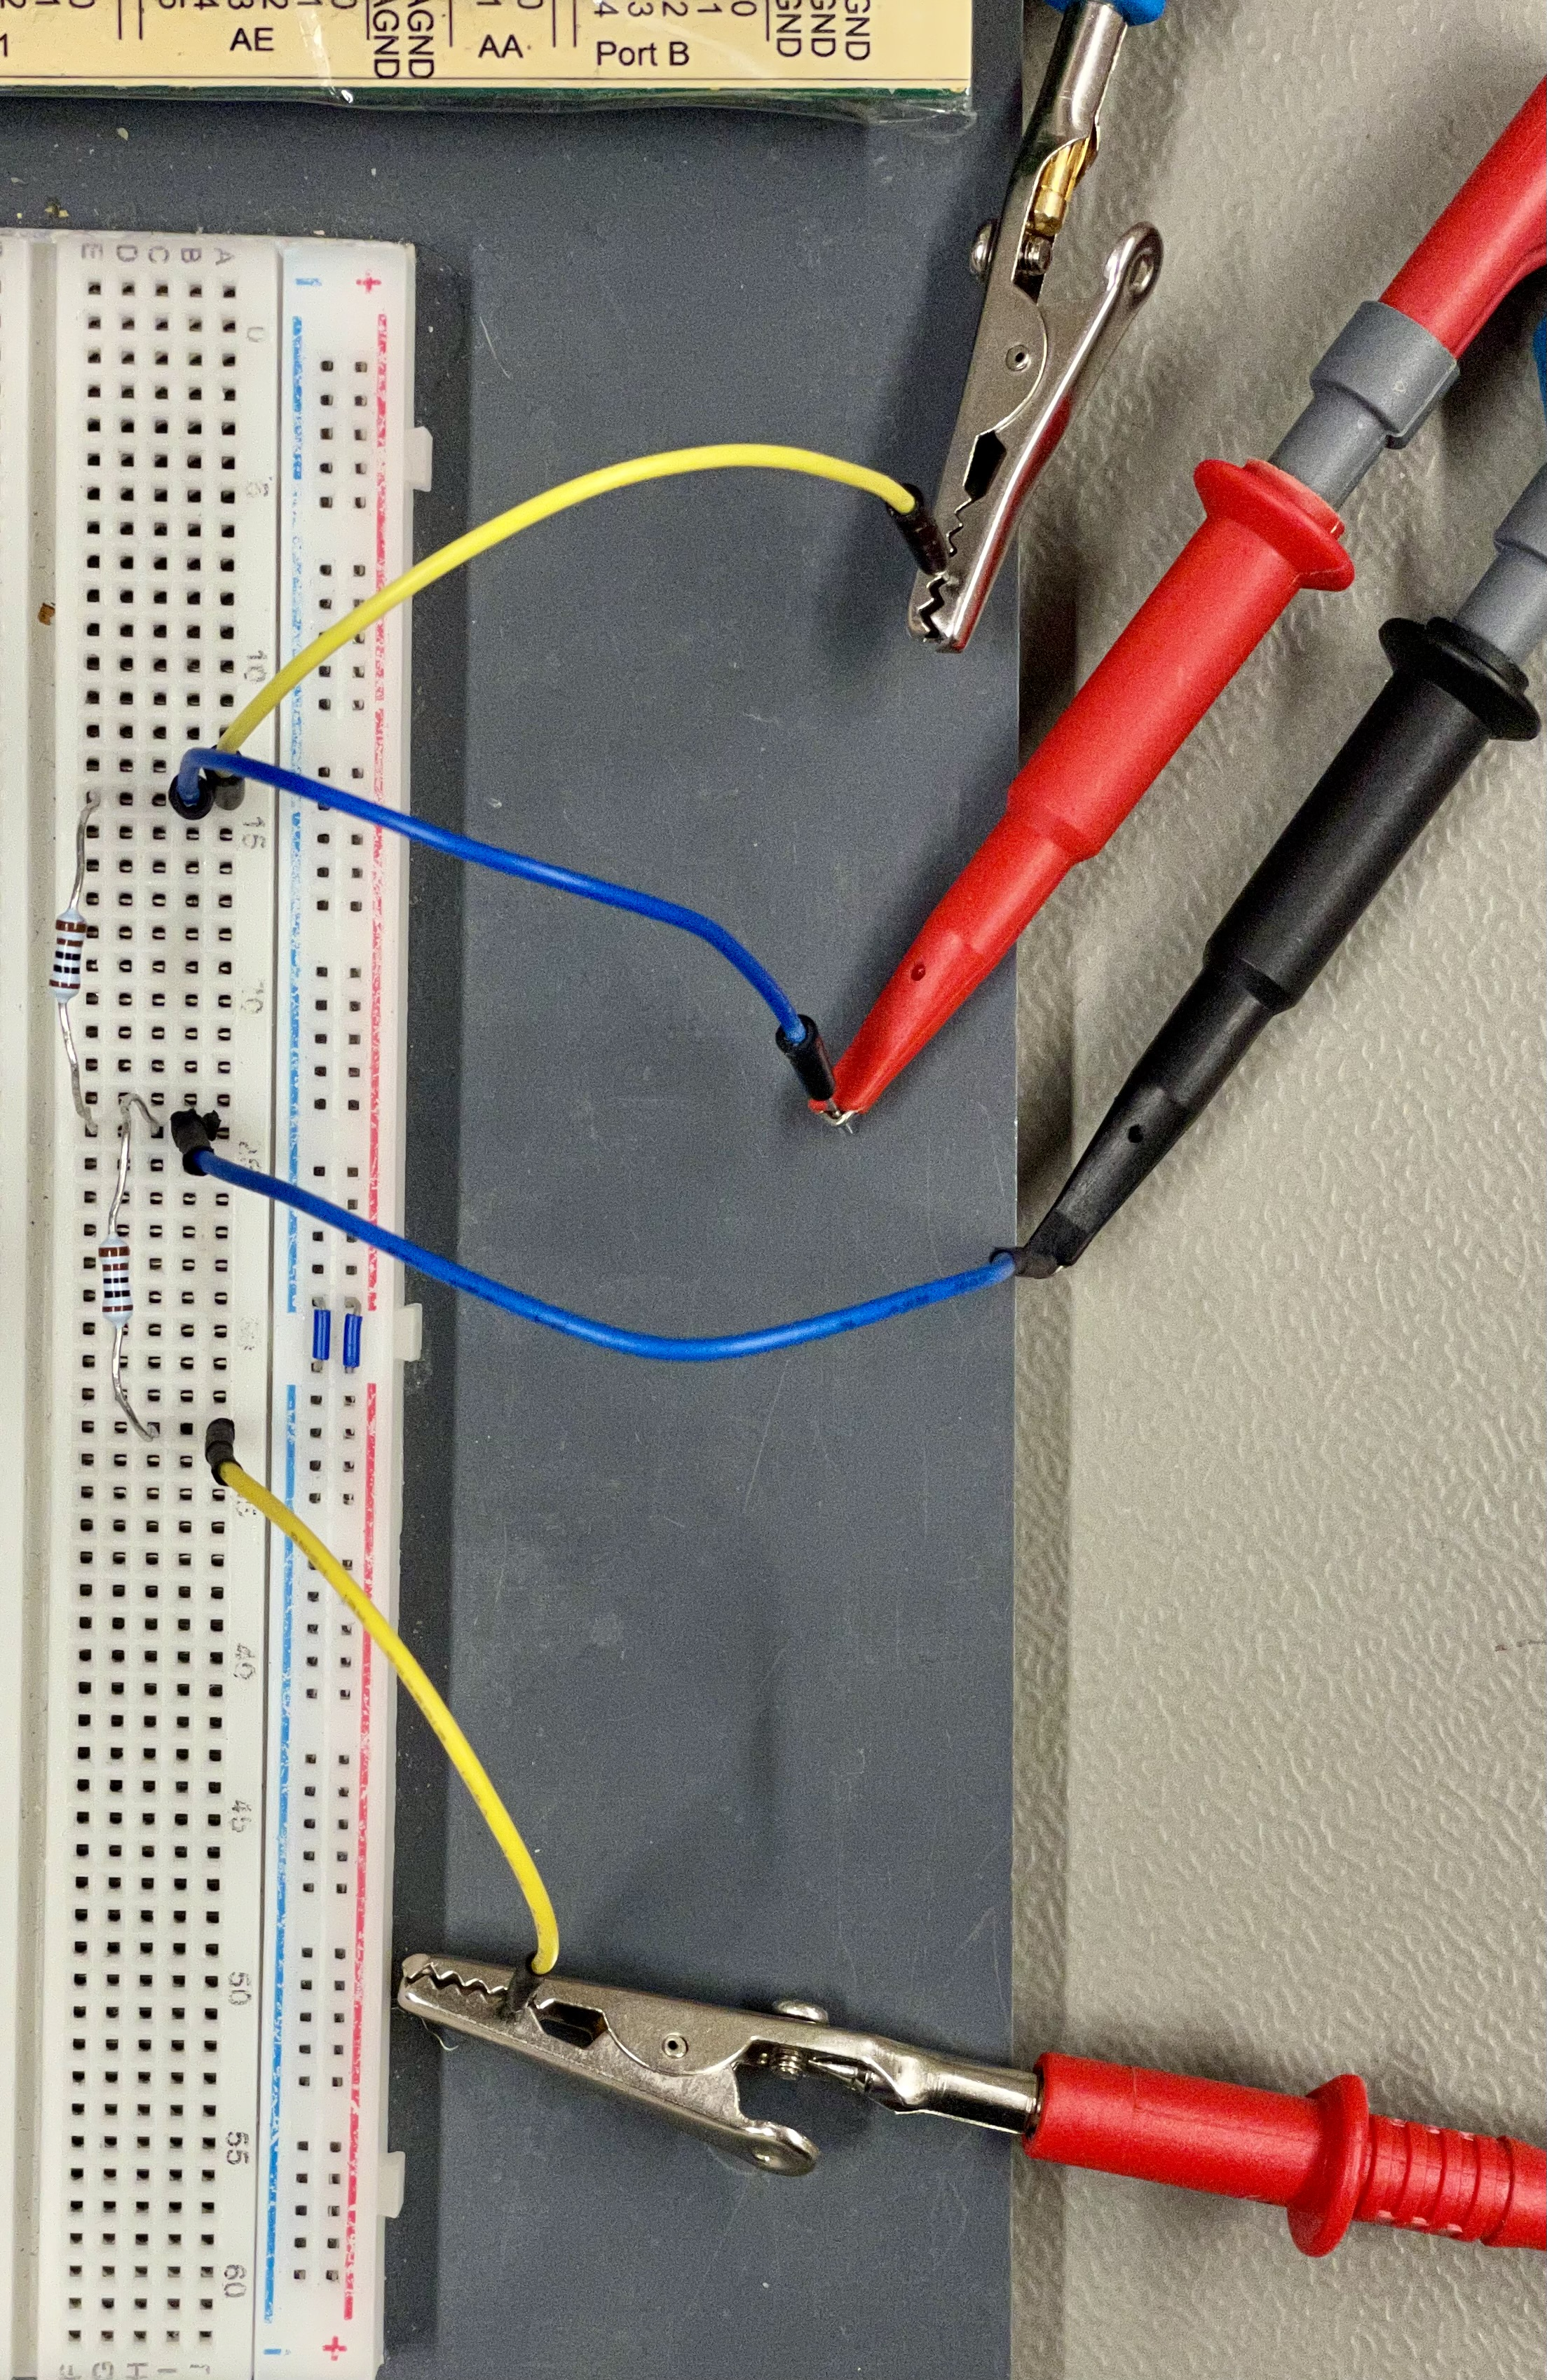
\includegraphics[width=\linewidth]{task7-2-2-0.JPG}
		\caption{Messpunkt 2}
		\label{task7-2-2-0}
	\end{minipage}
	\hfill
	\begin{minipage}[c]{0.32\linewidth}
		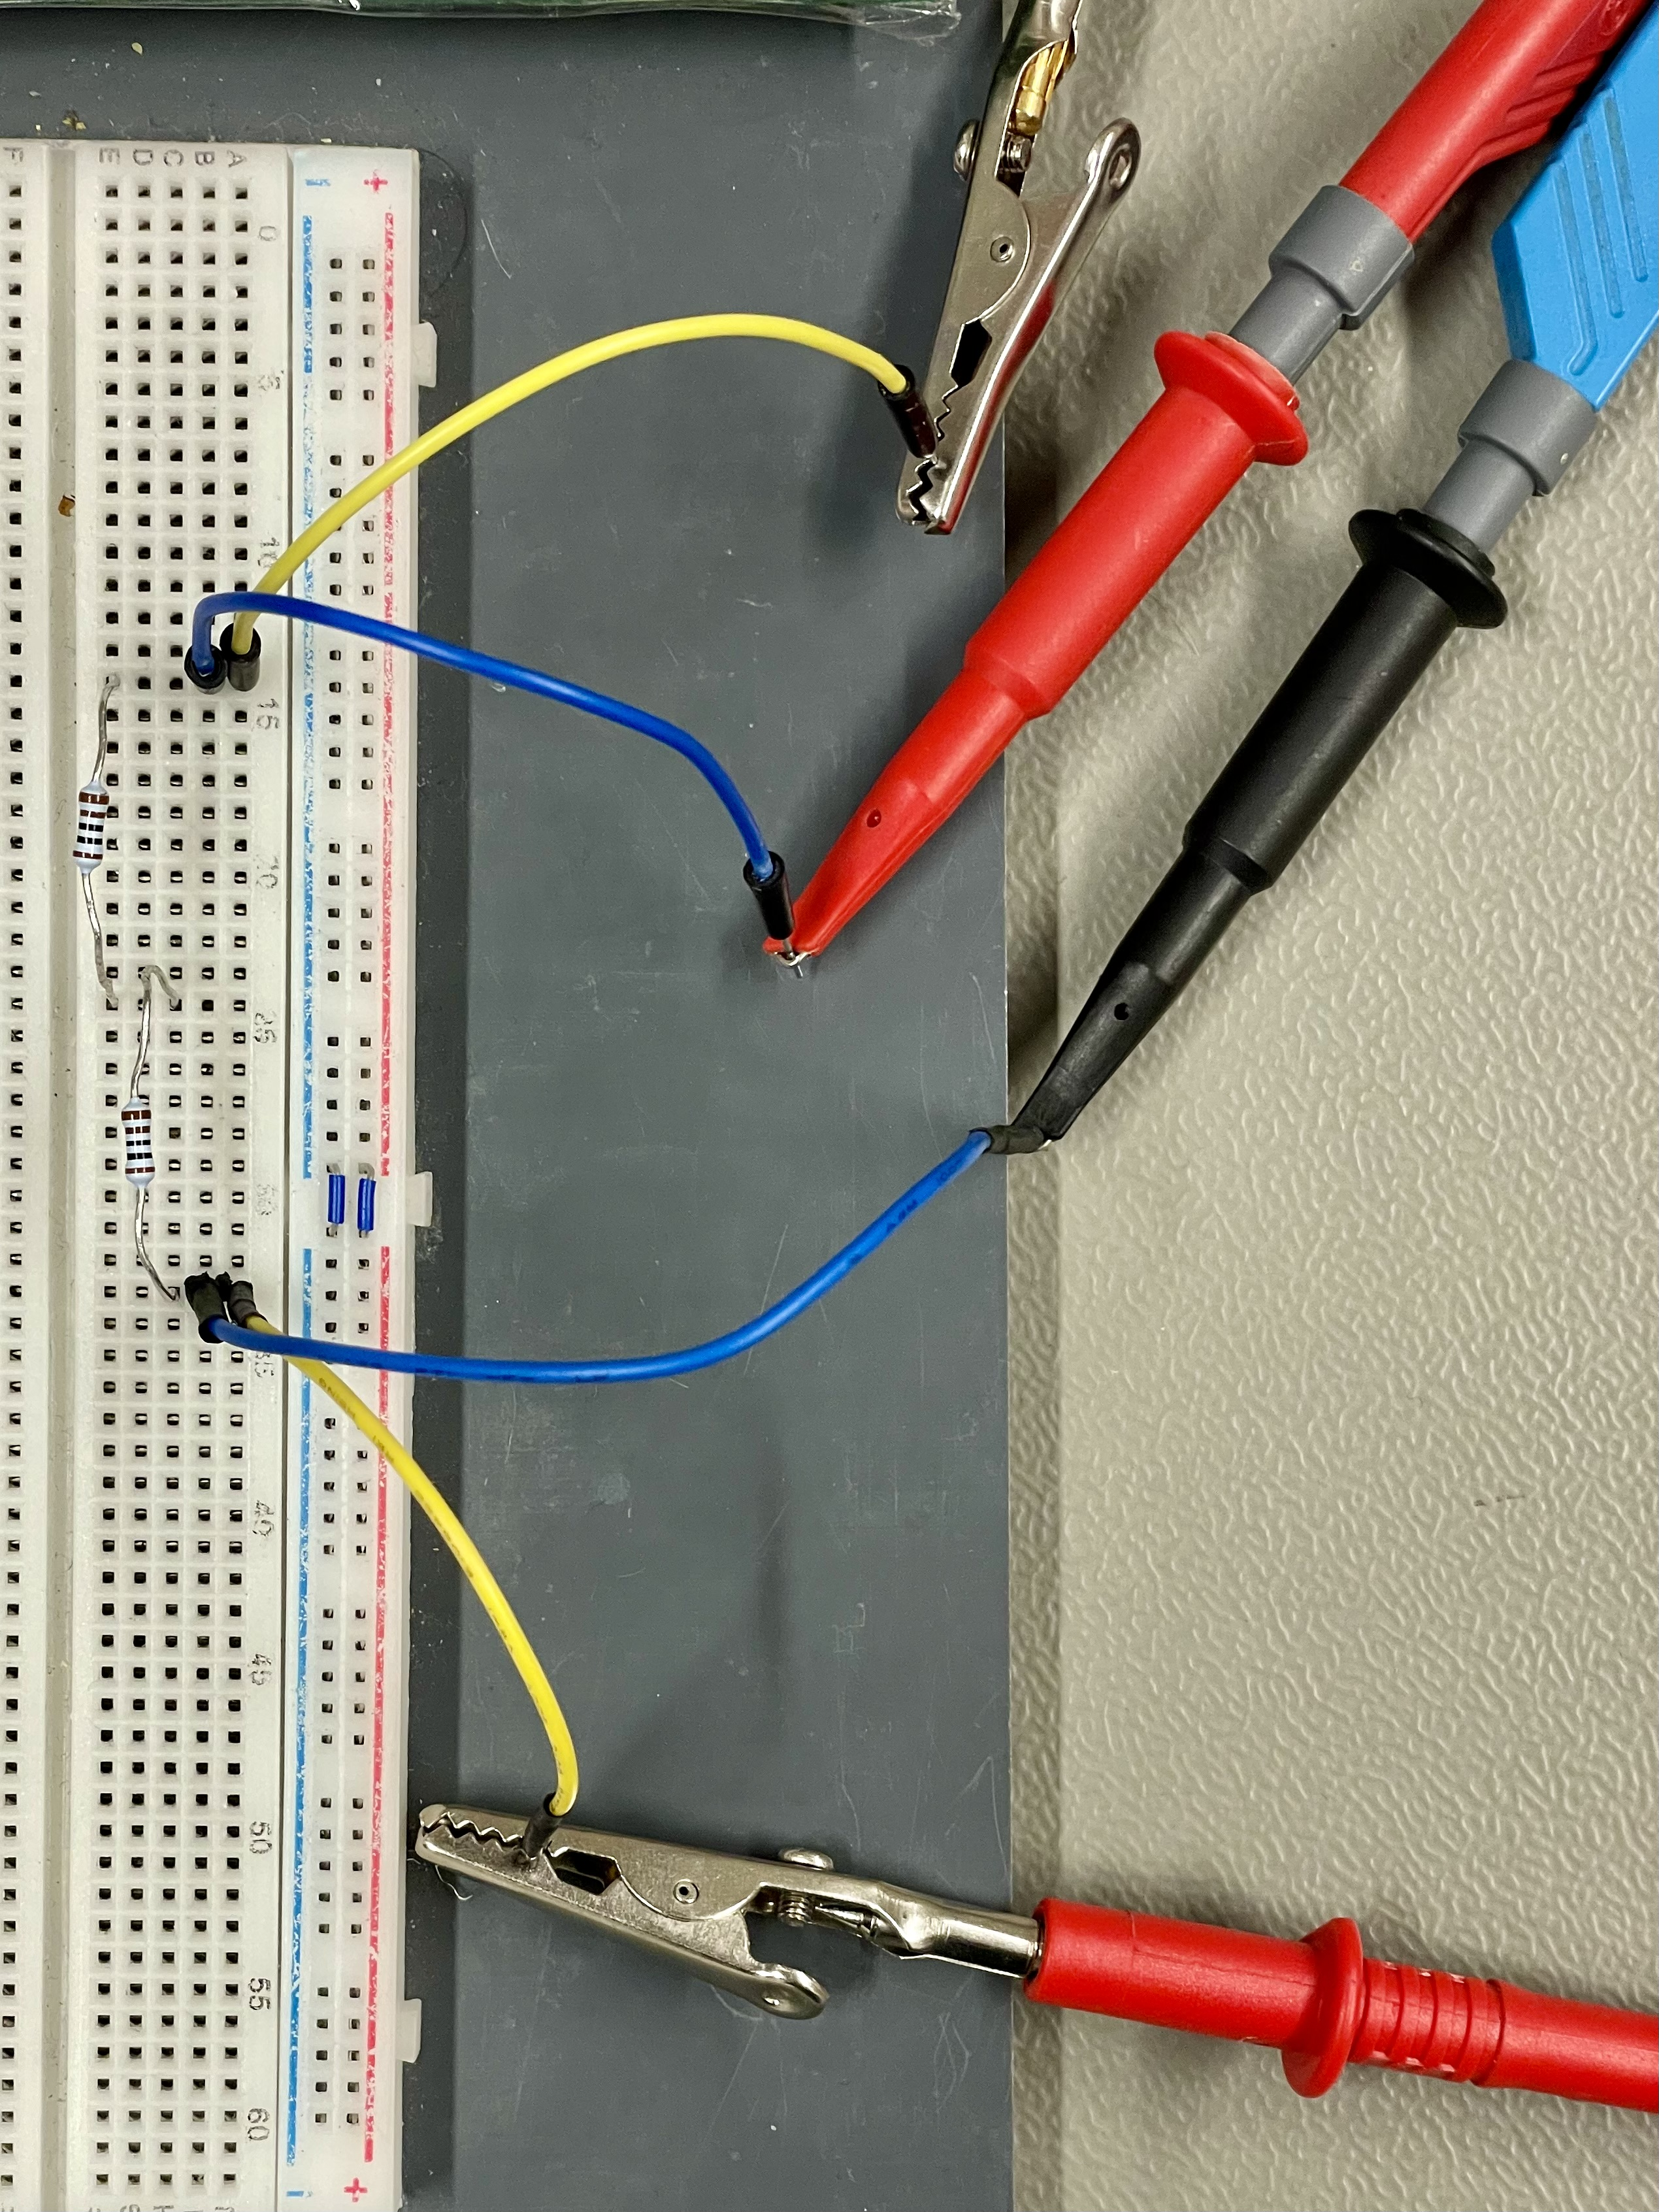
\includegraphics[width=\linewidth]{task7-2-3-0.JPG}
		\caption{Messpunkt 3}
		\label{task7-2-3-0}
	\end{minipage}
	\caption{Aufbau Messpunkte}
	\label{task7-2-1-aufbau}
\end{figure}

\begin{figure}
	\begin{minipage}[c]{0.48\linewidth}
		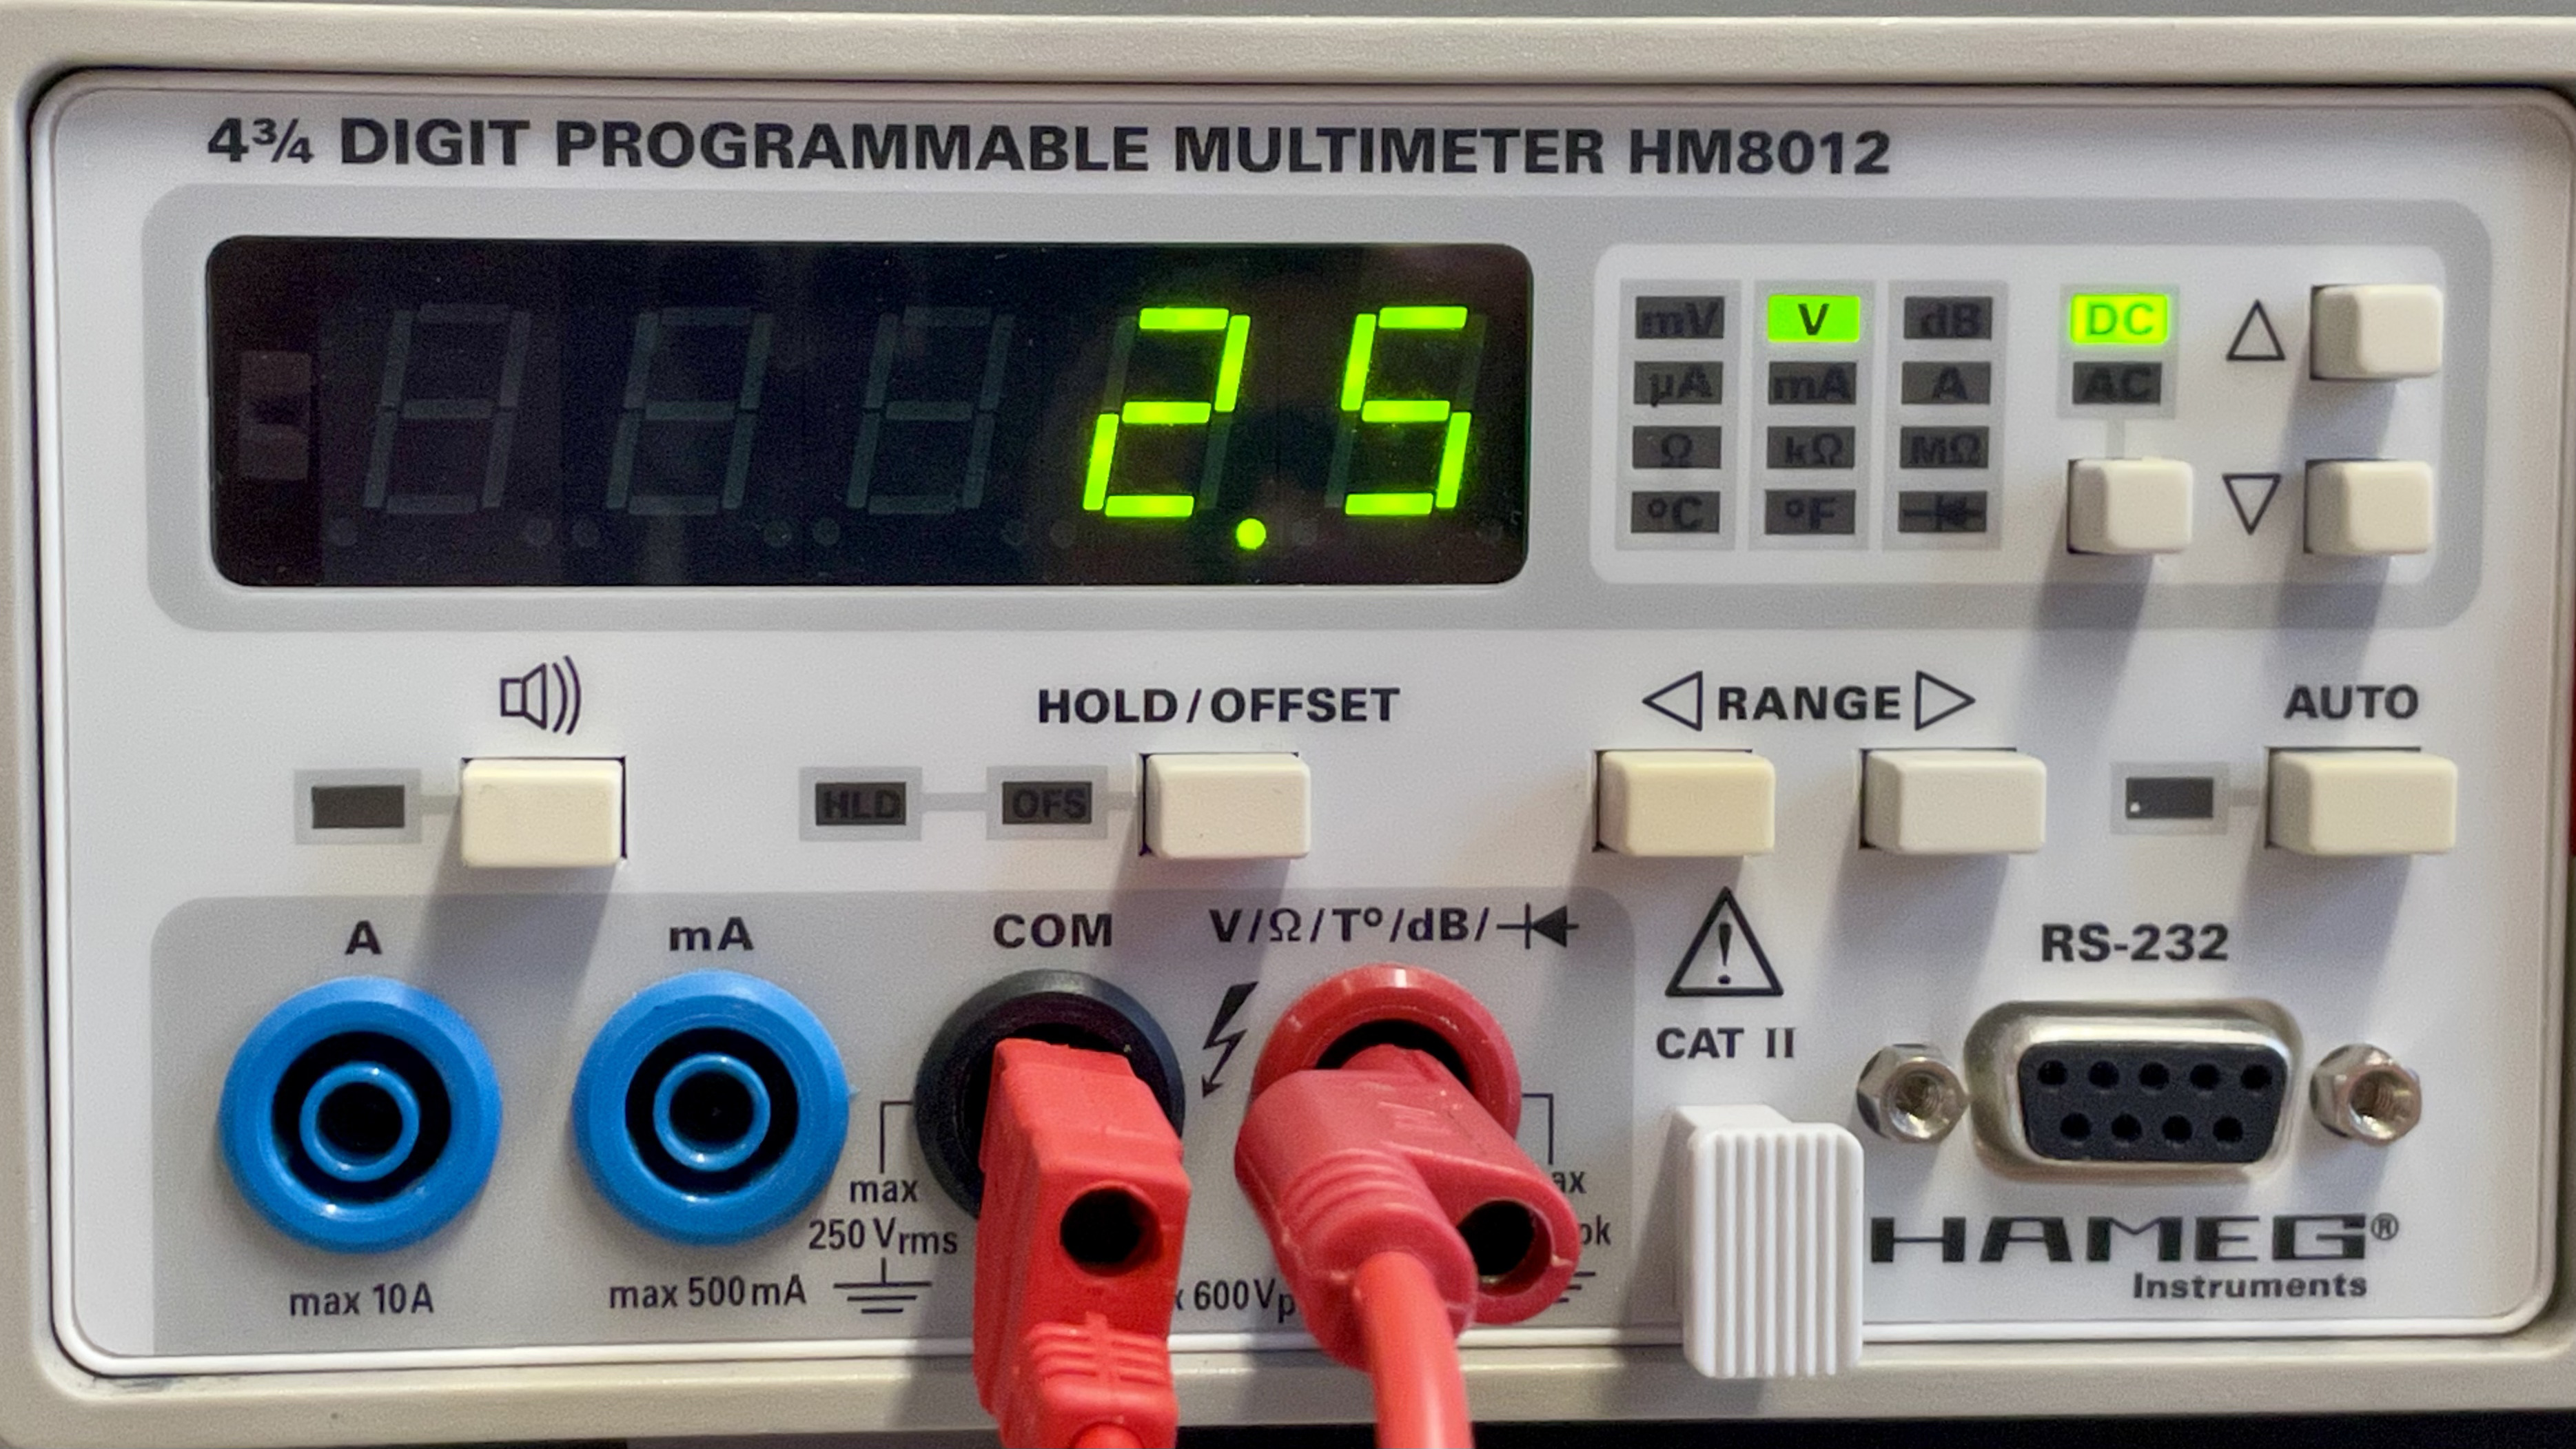
\includegraphics[width=\linewidth]{task7-2-2-1.JPG}
		\caption{Messpunkt 2}
		\label{task7-2-2-1}
	\end{minipage}
	\hfill
	\begin{minipage}[c]{0.48\linewidth}
		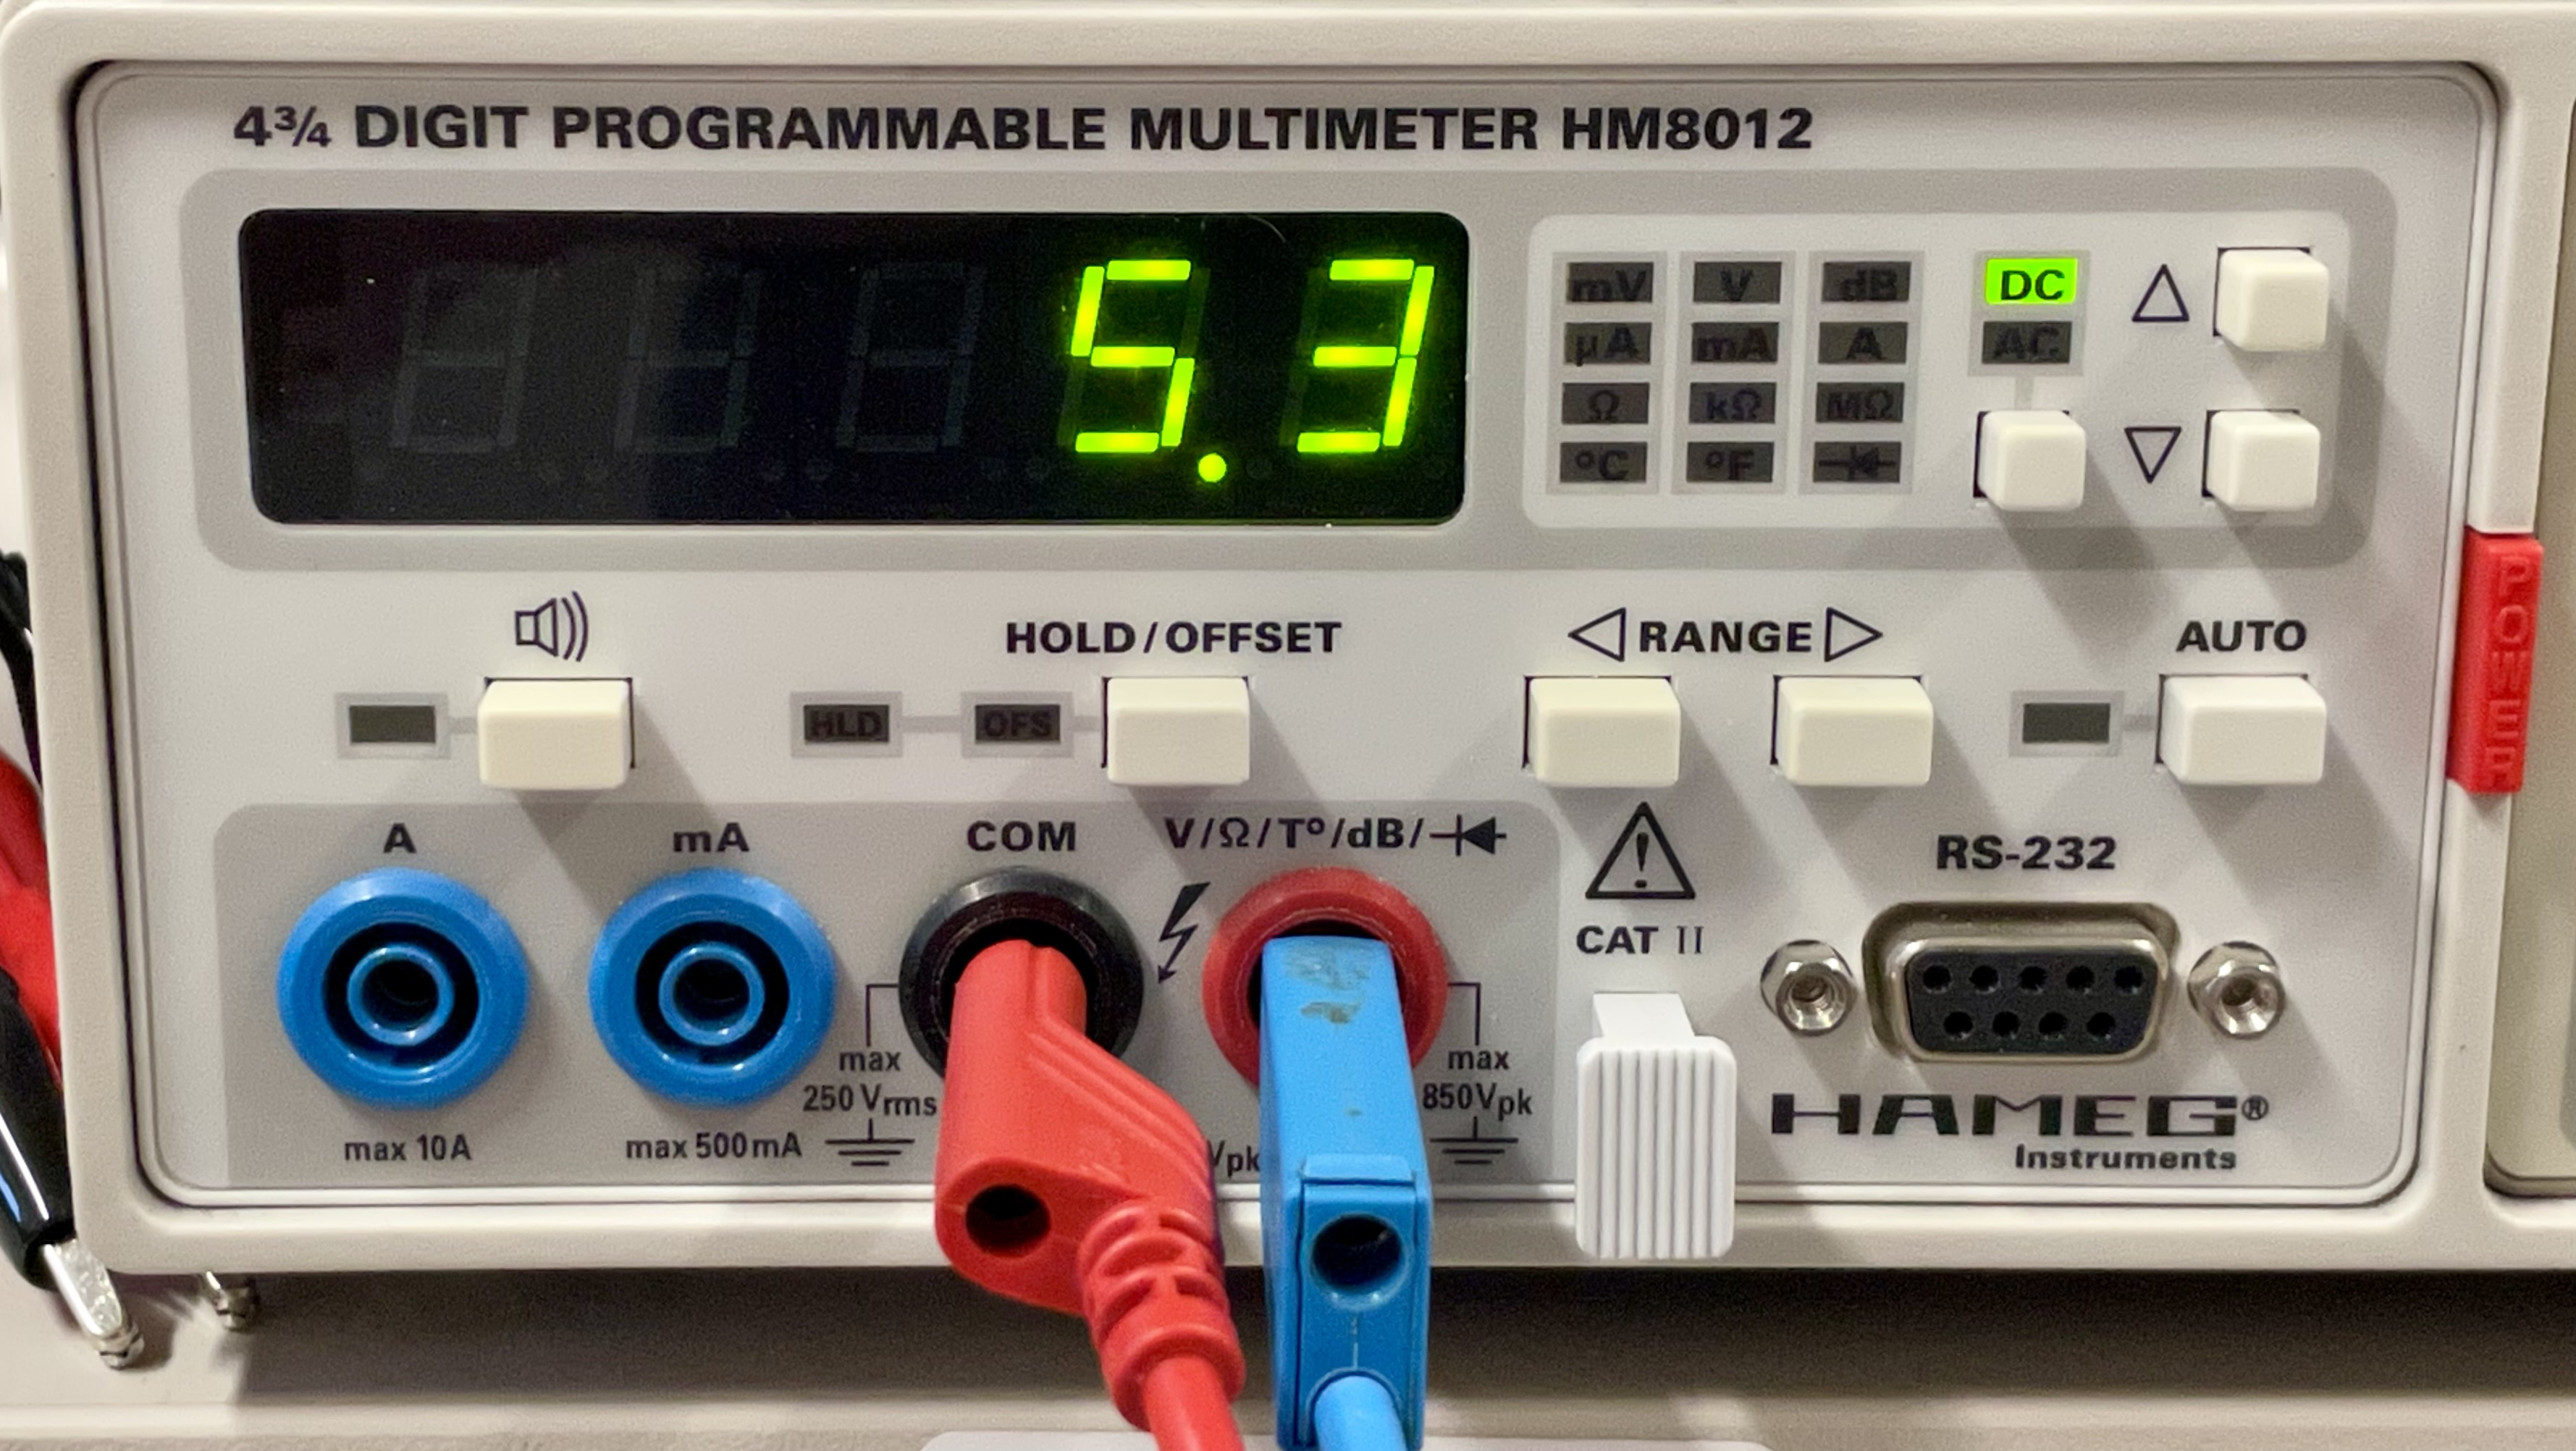
\includegraphics[width=\linewidth]{task7-2-3-1.JPG}
		\caption{Messpunkt 3}
		\label{task7-2-3-1}
	\end{minipage}
	\caption{Messwerte Messpunkte}
	\label{task7-2-1-messwerte}
\end{figure}

\section{Aufgabe 7.3}
\paragraph{Aufgabenstellung}
Ermitteln Sie rechnerisch Erwartungswerte für Strom und Spannung!

\paragraph{Durchführung}
Berechnen lassen sich nur Messpunkt 1 und 2. Messpunkt 3 hat zwischen sich und der Spannungsquelle keinen Abnehmer, daher wird hier direkt die Eingangsspannung gemessen. \\
\[I=\frac{U}{R}=\frac{\SI{5}{\volt}}{\SI{2}{\kilo\ohm}}=\SI{2,5}{\milli\ampere}\] \\
\[U=R*I=\SI{1}{\kilo\ohm}*\SI{2,5}{\milli\ampere}=\SI{2,5}{\volt}\]

\section{Aufgabe 7.4}
\paragraph{Aufgabenstellung}
Stellen Sie eine Hypothese zu den aufgetretenen Abweichungen auf!

\paragraph{Durchführung}
Die analogen Anzeigen zum einstellen von Strom und Spannung sind ungenauer als digitale Anzeigen und es können Abweichung auftreten, wenn diese nicht geeicht oder kalibriert sind. Der Widerstand des Steckbretts spielt ebenfalls eine Rolle, da dieser durch z.B. Korrosion die Messwerte beeinflussen kann.